%=============================================================================
% extdrift — IEEE conference paper (compile on Overleaf with pdfLaTeX)
% Self-contained: TikZ + pgfplots figures, no external image files needed.
% NOTE: verify/complete the bibliography details before submission.
%=============================================================================
\documentclass[conference]{IEEEtran}
\IEEEoverridecommandlockouts

\usepackage{cite}
\usepackage{amsmath,amssymb,amsfonts}
\usepackage{algorithmic}
\usepackage{graphicx}
\usepackage{textcomp}
\usepackage{xcolor}
\usepackage{booktabs}
\usepackage{array}
\usepackage{url}
\usepackage{tikz}
\usetikzlibrary{arrows.meta,positioning,shapes.geometric,calc}
\usepackage{pgfplots}
\pgfplotsset{compat=1.17}

\def\BibTeX{{\rm B\kern-.05em{\sc i\kern-.025em b}\kern-.08em
    T\kern-.1667em\lower.7ex\hbox{E}\kern-.125emX}}

\begin{document}

\title{Scoring the Change, Not the Extension:\\
Dynamic Behavioural Differencing for Detecting\\
Malicious Browser-Extension Updates}

\author{
\IEEEauthorblockN{Bind Pratap Singh}
\IEEEauthorblockA{\textit{Dept. of Computer Science and Engineering}\\
\textit{Shiv Nadar Institution of Eminence}\\
Delhi-NCR, India \\
bs563@snu.edu.in}
\and
\IEEEauthorblockN{Suhani Deepak Agrawat}
\IEEEauthorblockA{\textit{Dept. of Computer Science and Engineering}\\
\textit{Shiv Nadar Institution of Eminence}\\
Delhi-NCR, India}
\and
\IEEEauthorblockN{Sweta Mishra}
\IEEEauthorblockA{\textit{Dept. of Computer Science and Engineering}\\
\textit{Shiv Nadar Institution of Eminence}\\
Delhi-NCR, India}
}

\maketitle

\begin{abstract}
Browser extensions run with deep access to the pages a user visits, their cookies, and their
form data, and they update themselves \emph{silently and automatically}. This creates a
supply-chain risk that store review is not designed to catch: an extension that is benign for
years can turn malicious in a single update, as in the December~2024 Cyberhaven incident.
We present \textbf{extdrift}, a system that detects malicious \emph{updates} rather than
malicious extensions by \emph{differencing behaviour} across two consecutive versions:
$\Delta = f(v_2) - f(v_1)$, where $f(\cdot)$ is a feature vector derived from what each version
\emph{does} when executed in a sealed, deterministic sandbox. Because the method observes
runtime effects rather than source text, it is robust to code obfuscation that blinds static
analysis. extdrift instruments both content scripts and the Manifest~V3 service worker across a
Chromium and a Firefox capture engine sharing one trace schema, elicits dormant payloads with a
HoneyPage and event-handler fuzzing, and scores each delta with three complementary layers:
transparent rules, a gradient-boosted-tree classifier selected by a leakage-free bake-off, and a
benign-trained anomaly detector for unseen threats. On a hardened corpus, the learned model
reduces the false-positive rate at 90\% recall from 45\% (rules) to under 2\%, a gain that is
statistically significant (bootstrap 95\% CI $[0.093, 0.137]$ in PR-AUC). Trained on synthetic
data \emph{only} and evaluated on 45 held-out captures from 15 real extensions never seen in
training, it attains PR-AUC~0.998 at precision~1.0, demonstrating transfer to the real world. A
head-to-head on 21 real extensions shows a static update-diff detector catches a clean payload
21/21 but an obfuscated one 0/21, while our dynamic diff catches both. We also quantify, and are
explicit about, the central data-availability constraint: real malicious \emph{update pairs}
cannot be sourced from public repositories (we measure 60\% of known-malicious IDs delisted and
0/15 with archived predecessors), which motivates a principled real-extension-weaponisation
substitute.
\end{abstract}

\begin{IEEEkeywords}
browser extension security, malicious update detection, dynamic analysis, behavioural
differencing, software supply chain, machine learning, anomaly detection
\end{IEEEkeywords}

%=============================================================================
\section{Introduction}
%=============================================================================
Browser extensions are among the most privileged software a typical user installs. Once granted
permissions, an extension can read the content of every page the user opens, exfiltrate cookies
(which are live authenticated sessions), capture keystrokes and form fields, observe browsing
history, and rewrite pages before rendering. Hundreds of millions of users install extensions
from the Chrome Web Store and Mozilla Add-ons (AMO) and then rarely revisit that decision,
because extensions \emph{update automatically and silently}: after the initial installation, new
code arrives on the user's machine without further review or consent.

This auto-update channel is a supply-chain attack surface. An extension can be honest for years
and then turn malicious in a single update---because the developer sold the extension, their
store account was phished, or a build dependency was compromised. The December~2024 Cyberhaven
incident~\cite{cyberhaven} is the canonical example: a phished developer account pushed a
malicious update to a widely deployed, legitimate extension, which then exfiltrated session
tokens from everyone whose browser auto-updated. Earlier cases such as
DataSpii~\cite{dataspii} and large-scale ad-injection campaigns~\cite{palant} follow the same
bait-and-switch-on-update pattern, frequently as \emph{adware}: ad injection, affiliate-link
hijacking, and data collection stapled onto a formerly clean extension.

Store review largely evaluates an extension in isolation and at a point in time. It is not
designed to reason about \emph{what changed between two consecutive versions and whether that
change is dangerous}. That specific gap---the malicious \emph{update}, not the malicious
\emph{extension}---is what this work targets.

\noindent\textbf{Approach.} Our central idea is to \emph{score the change, not the extension}. A
password manager reads passwords in \emph{every} version; that alone is never suspicious. What is
suspicious is an update that \emph{newly starts} sending that data to a server the extension
never previously contacted. For two consecutive versions $v_1$ (trusted baseline) and $v_2$
(candidate update) we compute a behaviour feature vector $f(\cdot)$ for each and take the
behavioural delta $\Delta = f(v_2) - f(v_1)$; the label lives in the change. Crucially, we derive
$f(\cdot)$ from \emph{observed runtime behaviour}, so obfuscation that hides malicious code does
not hide the malicious \emph{effect}---a cookie read closely followed by an upload to a new host.

\noindent\textbf{Contributions.}
\begin{itemize}
\item A \emph{dynamic behavioural differencing} formulation for malicious-update detection, and a
sealed, deterministic sandbox that makes the diff meaningful by eliminating web noise while
sealing all egress.
\item A capture design that instruments content scripts, MV2 background pages, and the MV3 service
worker across \emph{two} browser engines (Chromium and Firefox) behind one trace schema, with a
HoneyPage and event-handler fuzzing to elicit trigger-dependent payloads.
\item A three-layer detector---transparent rules, a gradient-boosted classifier selected by an
evidence-based, leakage-free bake-off, and a benign-trained anomaly layer---evaluated with
extension-level grouping and a strict temporal split.
\item An honest treatment of data: we \emph{measure} the unavailability of real malicious update
pairs (delisting and lack of archived predecessors) and adopt a real-extension-weaponisation
substitute, then validate that a model trained on synthetic data transfers to real extensions.
\item An empirical reproduction, on 21 real extensions, of the obfuscation blind spot of static
update-differencing, which our dynamic method closes.
\end{itemize}

%=============================================================================
\section{Threat Model and Background}
%=============================================================================
\noindent\textbf{Assets and adversary.} The adversary controls the publishing account of an
extension already installed by many users, and pushes a malicious update through the legitimate
auto-update channel. The goal is data theft (cookies, credentials, browsing history), covert
ad/affiliate injection, or traffic redirection. We assume the attacker has full control over the
extension's own code but cannot bypass the browser's permission model, and that the malicious
behaviour manifests at runtime (possibly only under specific triggers). We treat \emph{adware}
that injects ads or collects data without consent as in scope, following documented incidents.

\noindent\textbf{Extension architecture.} A modern extension is multi-component: content scripts
run in the page, a background context (an MV2 page or an MV3 service worker) runs privileged
logic, and the two communicate by message passing. The MV3 service worker has no associated page,
making it a common analysis blind spot~\cite{karami}. An update can therefore split a kill chain
across components---a content script harvests data and hands it to the service worker, which
exfiltrates it---to evade single-component analysis.

\noindent\textbf{Why the problem is hard.} A naive comparison of two live browsing sessions is
dominated by web noise (ads, nonces, timestamps) unrelated to the extension. Malicious behaviour
must be \emph{elicited} rather than merely awaited~\cite{hulk}. Static code-differencing is
defeated by obfuscation~\cite{youvechanged}. Finally, no public labelled corpus of malicious
\emph{update pairs} exists, and---as we quantify in Section~\ref{sec:data}---such pairs cannot be
assembled from public sources.

%=============================================================================
\section{Related Work}
%=============================================================================
\noindent\textbf{Update differencing.} \emph{You've Changed}~\cite{youvechanged} detects malicious
extensions by comparing the code of consecutive versions and clustering the additions. It is the
closest prior work and our conceptual anchor, but it is \emph{static}: obfuscation of the added
code hides the tells. Our method differs the \emph{behaviour} of consecutive versions, which is
robust to obfuscation; we adopt You've Changed's empirically most-discriminative API/sink
vocabulary for our static baseline and reproduce its obfuscation limitation on real code
(Section~\ref{sec:eval}).

\noindent\textbf{Dynamic analysis of extensions.} Hulk~\cite{hulk} pioneered eliciting malicious
extension behaviour with HoneyPages and event-handler fuzzing on \emph{single} versions; we adopt
these techniques and apply them across a version \emph{pair}. VEX~\cite{vex} statically vets
extensions for vulnerabilities. Work on extension message passing such as
EmPoWeb~\cite{empoweb} motivates our cross-component features.

\noindent\textbf{Malicious-domain signals.} Lexical domain-reputation features from DGA
detection~\cite{antonakakis} inform our low-reputation-destination feature.

Relative to this body of work, our contribution is the combination of (i) \emph{behavioural}
(not static) update-differencing, (ii) a sealed deterministic sandbox with cross-engine,
cross-manifest instrumentation, and (iii) a rigorously evaluated three-layer detector whose
synthetic training transfers to real extensions.

%=============================================================================
\section{Approach Overview}
%=============================================================================
Figure~\ref{fig:pipeline} shows the pipeline. A \texttt{.crx}/\texttt{.xpi} package is unpacked;
each version is executed under an identical scripted scenario in the sandbox to produce a
validated \emph{trace}; the trace is reduced to $f(\cdot)$; the two vectors are subtracted to form
$\Delta$; and $\Delta$ is scored by three layers whose verdicts are combined into
\textsc{Benign}/\textsc{Suspicious}/\textsc{Malicious} with the exact new behaviours as evidence.
The analysis half (unpack $\rightarrow$ features $\rightarrow$ scoring) is pure and runs on
commodity hardware; only capture needs a browser.

\begin{figure}[t]
\centering
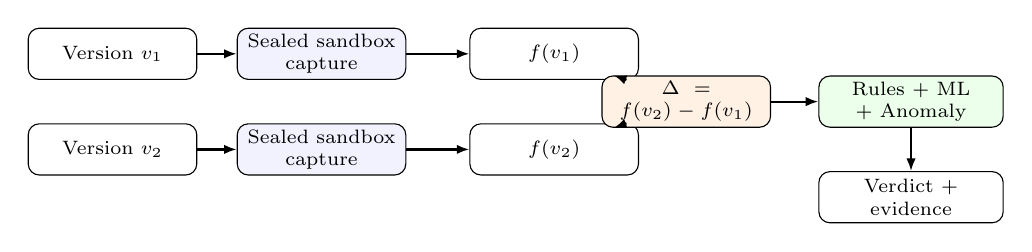
\begin{tikzpicture}[
  node distance=5.5mm and 5mm,
  box/.style={draw, rounded corners, align=center, font=\scriptsize,
              minimum height=6.5mm, inner sep=2pt, text width=20mm},
  arr/.style={-{Latex[length=1.6mm]}, thick}]
\node[box] (v1) {Version $v_1$};
\node[box, below=of v1] (v2) {Version $v_2$};
\node[box, right=of v1, fill=blue!5] (c1) {Sealed sandbox capture};
\node[box, right=of v2, fill=blue!5] (c2) {Sealed sandbox capture};
\node[box, right=8mm of c1] (f1) {$f(v_1)$};
\node[box, right=8mm of c2] (f2) {$f(v_2)$};
\coordinate (mid) at ($(f1)!0.5!(f2)$);
\node[box, right=6mm of mid, fill=orange!10] (d) {$\Delta = f(v_2)-f(v_1)$};
\node[box, right=6mm of d, fill=green!8, text width=22mm] (s)
     {Rules $+$ ML $+$ Anomaly};
\node[box, below=5.5mm of s, text width=22mm] (o)
     {Verdict $+$ evidence};
\draw[arr] (v1)--(c1); \draw[arr] (v2)--(c2);
\draw[arr] (c1)--(f1); \draw[arr] (c2)--(f2);
\draw[arr] (f1)--(d);  \draw[arr] (f2)--(d);
\draw[arr] (d)--(s);   \draw[arr] (s)--(o);
\end{tikzpicture}
\caption{The extdrift pipeline. Two consecutive versions are captured under an identical
scenario; their behavioural feature vectors are differenced; the delta is scored by three
layers into an explainable verdict.}
\label{fig:pipeline}
\end{figure}

%=============================================================================
\section{Deterministic Behavioural Capture}
%=============================================================================
The soundness of a behavioural diff rests entirely on the two versions seeing an
\emph{identical} world, so that the extension version is the only variable.

\noindent\textbf{Determinism.} An in-process server returns byte-identical responses for a fixed
set of hosts under the reserved \texttt{.test} TLD (a fake bank, a webmail inbox, and a
HoneyPage). The Chromium engine maps every \texttt{.test} name to this server via
\texttt{-{}-host-resolver-rules}; the Firefox engine, which lacks such a flag, is routed through a
local forward proxy that serves the same content. Both engines emit the same trace schema, so
Chromium/synthetic rows and Firefox/real rows are directly comparable.

\noindent\textbf{Safety.} All egress is intercepted. A synthetic exfiltration attempt reaches a
fake collector that logs the attempt as ground truth for a leak, but no data leaves the machine.
Real extensions are analysed locally and their code is never redistributed.

\noindent\textbf{Instrumentation.} We never analyse original files. A scratch copy is made and a
small JavaScript prelude is prepended to every script the manifest loads---content scripts, MV2
background pages, and MV3 service workers. The prelude hooks security-relevant APIs
(\texttt{document.cookie}, \texttt{fetch}/\texttt{XHR}/\texttt{sendBeacon},
\texttt{chrome.*}/\texttt{browser.*}) and reports each event over a sealed channel that the driver
strips from the trace. A notable engineering finding: in a Firefox content script,
\texttt{window} refers to the page's cross-origin-wrapped realm, whose \texttt{fetch} differs from
the one the content-script code actually invokes; hooking the wrong realm silently lost every
content-script event. Binding instrumentation to the current realm's global
(\texttt{globalThis}) resolved this and raised real-extension malicious recall from 70\% to 100\%.

\noindent\textbf{Elicitation.} An idle page reveals little~\cite{hulk}. A scripted scenario drives
a HoneyPage dense with the elements a data-stealing payload seeks (login form, credential and
card fields, a session cookie), fills them, then fuzzes event handlers by dispatching synthetic
\texttt{submit}/\texttt{input}/\texttt{click} events so dormant handlers fire without a real
navigation that would race the trace.

%=============================================================================
\section{Feature Engineering}
%=============================================================================
Each feature is cheap to compute, explainable in one sentence, and traceable to a documented
behaviour. Two complementary sets are used.

\noindent\textbf{Behavioural features (26).} Derived from the four observation channels of the
trace, plus derived flow features; Table~\ref{tab:features} summarises the groups. Two features
target evasion specifically: cross-component message passing (the multi-component kill-chain tell)
and a low-reputation-destination count (lexical DGA/NRD-like egress hosts). Three static
manifest-diff features (added high-risk permissions, escalation to broad host access, added host
permissions) complete a 29-column vector.

\noindent\textbf{Static-code features (27).} A browser-free vector counting security-relevant
API/sink/obfuscation tokens and permission shifts between versions---the You've Changed
methodology---used both as a baseline and to bring real extension \emph{code} into the pipeline
without a browser. We adopt the empirically most-discriminative token set from the You've Changed
corpus, including ad-injection, self-preservation (\texttt{setUninstallURL}, \texttt{uninstallSelf},
\texttt{webstore.install}), dynamic script writing, and broad data-access tokens.

\begin{table}[t]
\caption{Behavioural feature groups (26 features) and their motivation.}
\label{tab:features}
\centering
\footnotesize
\begin{tabular}{@{}p{13mm}p{36mm}p{22mm}@{}}
\toprule
\textbf{Channel} & \textbf{Representative features} & \textbf{Signal} \\
\midrule
Network & requests, distinct/third-party hosts, POSTs, upload bytes, encoded params,
worker-initiated, low-reputation hosts & Exfiltration to new/low-reputation hosts \\
DOM & reads, sensitive reads, identity reads, injections & Credential theft, ad injection \\
Storage & storage calls, cookie reads, whole-jar reads & Session-token theft \\
API & calls, distinct, high-risk, message passing & Privileged capability use, IPC evasion \\
Derived & exfil flows, third-party exfil flows & Read-then-upload taint proxy \\
\bottomrule
\end{tabular}
\end{table}

%=============================================================================
\section{Datasets}
\label{sec:data}
%=============================================================================
\noindent\textbf{Why synthetic data is necessary.} No public labelled corpus of malicious update
\emph{pairs} exists, and---we show empirically---such pairs cannot be assembled from public
repositories. The Chrome Web Store serves only the current version of an extension; there is no
public version history. Probing the official update endpoint for a random sample of a
7{,}382-entry known-malicious ID list, we find $\approx$60\% are delisted (no current version), and
for the surviving $\approx$40\%, a third-party historical archive contained an earlier version for
\emph{0 of 15} sampled IDs. Consequently a $(\text{benign }v_1 \rightarrow \text{malicious }v_2)$
real pair cannot be sourced. We therefore (i) generate a hardened synthetic corpus and (ii) adopt
a \emph{real-extension-weaponisation} substitute for the malicious class, then validate transfer.

\noindent\textbf{Synthetic corpus.} A generator produces schema-valid trace pairs at scale from 12
benign personas and 9 malicious payload families (cookie theft, credential theft, service-worker
beacon, ad affiliate, keylogger, history exfiltration, form-jacking, redirect hijack, clipboard
steal). It deliberately injects overlap so no single threshold separates the classes: per-run
count jitter; \emph{hard-benign} updates that add a new third-party host, permission, or analytics
POST; and \emph{stealth-malicious} updates that avoid permission escalation, exfiltrate small
payloads, or beacon to CDN-like hosts. Malicious samples are produced by a weaponiser that injects
\emph{real} JavaScript payloads into an extension's own files in clean and obfuscated variants
with identical runtime behaviour.

\noindent\textbf{Real data.} Firefox AMO exposes full version history with a direct download per
version, yielding real \emph{benign} update pairs; we crawl the store by popularity to collect
them. For the malicious class we weaponise these same real extensions. We additionally collect the
current version of real Chrome extensions via the official update endpoint (used to validate the
Chromium engine). Table~\ref{tab:dataset} summarises the composition; the bulk is synthetic by
necessity, but real data is present in the identical schema and drives the transfer evaluation.

\begin{table}[t]
\caption{Behavioural dataset composition (1{,}047 update pairs).}
\label{tab:dataset}
\centering
\footnotesize
\begin{tabular}{@{}lrl@{}}
\toprule
\textbf{Source} & \textbf{Pairs} & \textbf{Class} \\
\midrule
Synthetic (250 exts $\times$ 4 updates) & 1{,}000 & benign + malicious \\
Real extensions, weaponised (Firefox) & 30 & malicious \\
Real benign AMO updates (Firefox) & 15 & benign \\
Reference fixtures & 2 & benign + malicious \\
\midrule
\textbf{Total} & \textbf{1{,}047} & 449 mal / 598 benign \\
\bottomrule
\end{tabular}
\end{table}

%=============================================================================
\section{Detection Models}
%=============================================================================
\noindent\textbf{Tier 1: rules.} Twelve weighted rules (e.g., \emph{new exfiltration flow to a
third party}, \emph{new bulk cookie read}, \emph{high-risk permission escalation}) yield an
interpretable score and verdict, serving as a transparent control the learned model must beat.

\noindent\textbf{Tier 2: the bake-off.} We do not assume a model; we evaluate six approaches on
identical features---rules (control), logistic regression, random forest, XGBoost, scikit-learn
HistGradientBoosting, and an RBF SVM---and select by evidence. Evaluation is leakage-free:
StratifiedGroupKFold by extension id (all versions of one extension stay in one fold) and a strict
temporal split (train on earlier updates, test on later ones). The reported metrics are PR-AUC
(appropriate for imbalanced detection) and the false-positive rate at 90\% recall (the usability
metric); selection is by PR-AUC, tie-broken by lower FPR.

\noindent\textbf{Tier 3: anomaly.} An IsolationForest/One-Class-SVM ensemble trained on
\emph{benign} deltas only flags updates whose behaviour is anomalous, covering families never seen
in supervised training---the zero-day case a supervised model structurally cannot address.

%=============================================================================
\section{Evaluation}
\label{sec:eval}
%=============================================================================
We answer six research questions.

\subsection{RQ1: Does the learned model beat the rules?}
Table~\ref{tab:bakeoff} reports the bake-off under extension-level cross-validation. The
gradient-boosted-tree family (HistGradientBoosting and XGBoost) and random forest occupy the top
and are statistically indistinguishable ($\approx$0.982--0.983 PR-AUC). Decisively, at 90\% recall
the transparent rules incur a 45\% false-positive rate whereas the boosted model incurs under 2\%
(Fig.~\ref{fig:fpr}). Bootstrapping the leakage-free out-of-fold predictions (2{,}000 resamples)
places the winner at PR-AUC $0.983\,[0.976, 0.989]$ versus rules $0.868\,[0.844, 0.891]$; the
$+0.115$ gain has 95\% CI $[0.093, 0.137]$, excluding zero---so the improvement is statistically
significant, not noise. Under the strict temporal split the winner holds at PR-AUC~$\approx$0.97,
indicating generalisation to future updates rather than memorisation of past ones.

\begin{table}[t]
\caption{Model bake-off (extension-level cross-validation, 1{,}047 pairs).}
\label{tab:bakeoff}
\centering
\footnotesize
\begin{tabular}{@{}lccc@{}}
\toprule
\textbf{Model} & \textbf{PR-AUC} & \textbf{ROC-AUC} & \textbf{FPR@90\%\,rec.} \\
\midrule
HistGradientBoosting & \textbf{0.983} & 0.982 & \textbf{0.008} \\
XGBoost & 0.982 & 0.983 & 0.015 \\
Random Forest & 0.982 & 0.983 & 0.027 \\
SVM (RBF) & 0.972 & 0.977 & 0.028 \\
Logistic Regression & 0.972 & 0.975 & 0.062 \\
Rules (control) & 0.868 & 0.883 & 0.450 \\
\bottomrule
\end{tabular}
\end{table}

\begin{figure}[t]
\centering
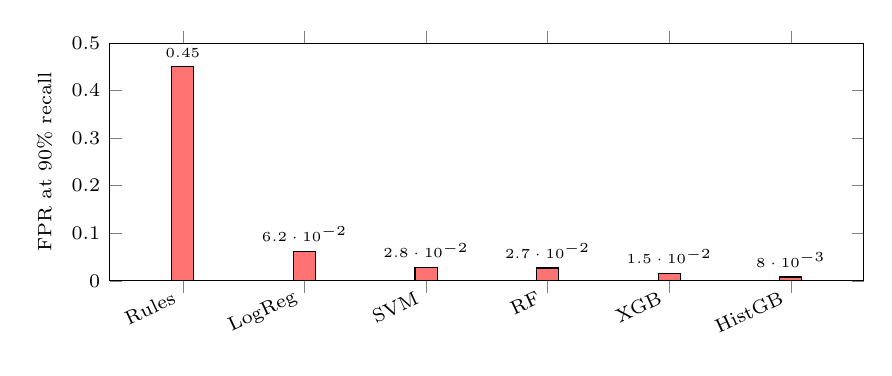
\begin{tikzpicture}
\begin{axis}[
  width=0.92\linewidth, height=4.6cm,
  ybar, bar width=8pt,
  ylabel={FPR at 90\% recall}, ymin=0, ymax=0.5,
  symbolic x coords={Rules,LogReg,SVM,RF,XGB,HistGB},
  xtick=data, x tick label style={font=\scriptsize,rotate=25,anchor=east},
  ytick={0,0.1,0.2,0.3,0.4,0.5}, ylabel style={font=\scriptsize},
  yticklabel style={font=\scriptsize}, enlarge x limits=0.12,
  nodes near coords, every node near coord/.append style={font=\tiny}]
\addplot[fill=red!55] coordinates
  {(Rules,0.450)(LogReg,0.062)(SVM,0.028)(RF,0.027)(XGB,0.015)(HistGB,0.008)};
\end{axis}
\end{tikzpicture}
\caption{False-positive rate to reach 90\% recall. The transparent rules flag 45\% of benign
updates; the gradient-boosted model flags under 2\%---the core case for the learned tier.}
\label{fig:fpr}
\end{figure}

\subsection{RQ2: Does synthetic training transfer to real extensions?}
This is the decisive question given a mostly-synthetic corpus. We train on synthetic data
\emph{only} and evaluate on 45 captured pairs from 15 real extensions (real benign updates and the
same extensions weaponised) that the model never saw. Table~\ref{tab:real} reports the result: the
transparent rules flag all 30 real weaponised updates (100\% recall), and the synthetic-only model
attains PR-AUC~0.998 at recall~0.93 and precision~1.0 with zero false positives on real benign
updates. A model that never observed a real extension separates real malicious updates from real
benign ones---empirical justification for the synthetic-data strategy. We further observe three
real benign updates that legitimately changed network behaviour and \emph{tripped a rule} (false
positives) yet were correctly classified benign by the learned model ($\le 0.03$ probability),
concretely illustrating the value of the learned tier over rules on real data. On a locked
by-extension held-out split (67 held-out extensions, threshold calibrated on the training portion
only), the model attains PR-AUC~0.976 with a 2\% FPR at 90\% recall, reported once.

\begin{table}[t]
\caption{Held-out evaluation on real extensions (45 pairs, 15 extensions).}
\label{tab:real}
\centering
\footnotesize
\begin{tabular}{@{}lc@{}}
\toprule
\textbf{Evaluation} & \textbf{Result} \\
\midrule
Rules: recall on real weaponised updates & 30/30 (100\%) \\
Synthetic-only model $\rightarrow$ real (held out) & PR-AUC 0.998 \\
\quad recall / precision / FPR & 0.93 / 1.00 / 0.00 \\
Anomaly (benign-only) on real, zero-shot & 28/30 (93\%), ROC-AUC 0.989 \\
\bottomrule
\end{tabular}
\end{table}

\subsection{RQ3: Static vs. dynamic under obfuscation}
We reproduce the static blind spot on real code. For each of 21 real extensions we inject the same
payload two ways---clean and obfuscated with identical runtime behaviour---and run a You've
Changed-style static detector on both. The static detector flags the clean injection in
\emph{21/21} cases but the obfuscated injection in \emph{0/21}: it is completely blinded by
obfuscation. Our dynamic diff flags both, because it observes the effect rather than the source.
This is the empirical case for dynamic behavioural differencing over static code-differencing.

\subsection{RQ4: Unseen threats}
Under leave-one-family-out evaluation the benign-trained anomaly layer flags entirely unseen
malicious families at 43--100\% (100\% on credential and cookie theft, lower on stealthy
families). Trained on synthetic-benign deltas only---never having seen a real extension or any
malicious example---it flags 28/30 (93\%) of real weaponised extensions at a 13\% false-positive
rate (ROC-AUC~0.989), demonstrating that the novelty layer transfers to the genuinely unseen.

\subsection{RQ5: Feature and data ablations}
A leave-one-group-out ablation confirms every channel earns its place: the DOM group contributes
the largest marginal PR-AUC, the network group is the most predictive in isolation ($\approx$0.89),
and the channels are complementary. A learning-curve analysis shows synthetic performance
plateaus near 0.97 PR-AUC by 400--800 pairs, indicating that further gains require real data
rather than more synthetic data. On the static track, semantic static-code features (PR-AUC~0.99
leave-one-extension-out) substantially outperform a raw token-churn baseline (0.81), with the
combination best (0.997), showing that security-aware tokens---not mere change magnitude---carry
the signal.

\subsection{RQ6: Cross-browser, MV3, and performance}
The Firefox engine is validated on 15 real extensions; the Chromium engine is validated on a real
Manifest~V3 extension end to end, with the service worker reached and a real-extension-turned-
malicious diff correctly classified \textsc{Malicious}. The analysis stage (delta plus scoring)
costs $\approx$0.22\,ms per pair, so once traces exist the detector scales to store size on a
single core; the browser-bound capture stage ($\approx$1--3\,min per version) is the only
bottleneck and parallelises across machines.

\subsection{Adware sub-study}
Adware (ad injection plus affiliate beaconing) is in scope. When the ad-injection family is
present in training it is detected within the main bake-off. As a stress test we hold the entire
family out: a supervised model does not extrapolate to this completely unseen family (0\% zero-shot
recall, its signature differing from the exfiltration families), but the benign-trained anomaly
layer still flags $\approx$49\% at a 1\% benign false-positive rate---reinforcing the rationale for
a separate novelty layer alongside the supervised classifier.

%=============================================================================
\section{Discussion and Limitations}
%=============================================================================
We are explicit about the constraints. First, no genuinely in-the-wild malicious update
\emph{pair} is captured; the malicious class is real-extension-weaponised because such pairs
cannot be sourced (RQ2 data, Section~\ref{sec:data}). The synthetic-to-real transfer result
mitigates but does not fully replace in-the-wild validation. Second, the real corpus (15
extensions, 45 pairs) is modest; a production false-positive claim warrants hundreds, which our
capture infrastructure supports but which is a matter of compute time. Third, although the
HoneyPage elicits most payloads, time-bomb and anti-analysis evasion remain open, and some
content-script payloads only fired after the realm fix. These are threats to validity we report
rather than obscure.

%=============================================================================
\section{Conclusion and Future Work}
%=============================================================================
extdrift detects malicious browser-extension \emph{updates} by differencing behaviour across
consecutive versions in a sealed, deterministic sandbox, and scoring the change with transparent
rules, a bake-off-selected gradient-boosted classifier, and a benign-trained anomaly layer. The
learned tier reduces false positives at 90\% recall from 45\% to under 2\% (a statistically
significant gain), a synthetic-only model transfers to real extensions at PR-AUC~0.998, and the
method closes the obfuscation blind spot that defeats static update-differencing on real code.
Future work includes scaling the real corpus to hundreds of extensions, a Tier-2 dependency-graph
neural model over cross-component message passing, and longitudinal collection to capture genuine
in-the-wild malicious updates.

%=============================================================================
\section*{Acknowledgment}
%=============================================================================
This work was carried out as an undergraduate research project (CSD493) at the Shiv Nadar
Institution of Eminence. All malicious samples are synthetic or executed in a sealed sandbox; no
third-party extension code is redistributed.

%=============================================================================
\begin{thebibliography}{00}
\bibitem{cyberhaven} Cyberhaven, ``Cyberhaven's Chrome extension security incident and what we're
doing about it,'' Technical incident report, Dec. 2024.
\bibitem{youvechanged} N. Pantelaios, N. Nikiforakis, and A. Kapravelos, ``You've Changed:
Detecting Malicious Browser Extensions through their Update Deltas,'' in \emph{Proc. ACM SIGSAC
Conf. Computer and Communications Security (CCS)}, 2020.
\bibitem{hulk} A. Kapravelos, C. Grier, N. Chachra, C. Kruegel, G. Vigna, and V. Paxson, ``Hulk:
Eliciting Malicious Behavior in Browser Extensions,'' in \emph{Proc. USENIX Security Symp.}, 2014.
\bibitem{empoweb} D. F. Som\'e, ``EmPoWeb: Empowering Web Applications with Browser Extensions,''
in \emph{Proc. IEEE Symp. Security and Privacy (S\&P)}, 2019.
\bibitem{vex} S. Bandhakavi, S. T. King, P. Madhusudan, and M. Winslett, ``VEX: Vetting Browser
Extensions for Security Vulnerabilities,'' in \emph{Proc. USENIX Security Symp.}, 2010.
\bibitem{karami} S. Karami, P. Ilia, and J. Polakis, ``Awakening the Web's Sleeper Agents:
Misusing Service Workers for Privacy Leakage,'' in \emph{Proc. Network and Distributed System
Security Symp. (NDSS)}, 2021.
\bibitem{antonakakis} M. Antonakakis \emph{et al.}, ``From Throw-Away Traffic to Bots: Detecting
the Rise of DGA-Based Malware,'' in \emph{Proc. USENIX Security Symp.}, 2012.
\bibitem{dataspii} S. Jadali, ``DataSpii: The catastrophic data leak via browser extensions,''
Technical report, 2019.
\bibitem{palant} W. Palant, ``Analysis of malicious/ad-injecting browser extensions,'' Technical
report, 2023.
\end{thebibliography}

\end{document}
